% !TEX spellcheck = en_US

\documentclass[conference]{IEEEtran}
\usepackage{cite}
\usepackage{amsmath,amssymb,amsfonts}
\usepackage{algorithmic}
\usepackage{graphicx}
\usepackage{textcomp}
\usepackage{xcolor}
% add hyperlinks, delete all .aux files if adding hyperref after previous build
\usepackage{hyperref}
% support for unicode charcters like "é" and "ñ"
\usepackage[T1]{fontenc}
% Provides generic commands \degree, \celsius, \perthousand, \micro and \ohm
\usepackage{gensymb}
% splits a section into multiple columns
\usepackage{multicol}
\def\BibTeX{{\rm B\kern-.05em{\sc i\kern-.025em b}\kern-.08em
    T\kern-.1667em\lower.7ex\hbox{E}\kern-.125emX}}
\begin{document}

\title{Tracker Terrain Loss Part Two}

\author{\IEEEauthorblockN{MinWah Leung, Mark A. Mikofski, Mike Hamer, Anja Neubert, Abhishek Parikh, Patrick Rainey,}
\IEEEauthorblockN{and Rounak Kharait}
	\IEEEauthorblockA{DNV, Oakland, CA, 94612, USA }}

\maketitle

\begin{abstract}
Trackers on variable terrain can incur electric mismatch losses from row-to-row shading even with backtracking. Tracker terrain loss is the difference between the performance of trackers on horizontal ground and that on variable terrain. SolarFarmer was used to study tracker terrain loss by simulating the Hopewell Friends Solar power plant, which has an average 4\% southwest slope. The results yielded a tracker terrain loss of -2\% with standard backtracking but slope-aware backtracking completely recovered the 2\% loss. By subdividing the site from one to three layouts, the tracker terrain loss decreased 0.5\%. The 1-hour versus 5-minute input data did not significantly affect the tracker terrain loss. This study is a continuation of a previous study that prompted improvements in SolarFarmer's 3-dimensional tracker shading algorithm. The results of this study demonstrate that SolarFarmer can now be used to calculate tracker terrain loss. A comparison of the SolarFarmer results with a separate uneven terrain model developed by DNV using PVsyst produced similar results.
\end{abstract}

\begin{IEEEkeywords}
trackers, terrain, losses, backtracking
\end{IEEEkeywords}

\section{Introduction}
Trackers increase energy output of PV systems by following the sun, maximizing the area of sunlight incident on the modules. However, most silicon modules are susceptible to electrical mismatch caused by uneven shade. Therefore, trackers typically "backtrack" to avoid  row-to-row shade occurring after sunrise and before sunset. Backtracking algorithms exist for horizontal ground ("standard backtracking") and uniformly sloped ground ("slope-aware backtracking"), which are described by closed-form expressions \cite{Marion2013,Anderson2020}. However, there is no general solution for terrain with variable, non-uniform slopes. If these backtracking algorithms are used for trackers on variable terrain, then row-to-row shading will occur, and typical silicon modules will incur electrical mismatch losses. 

In particular, standard backtracking on east-west (E-W) slopes causes shade loss at one end of the day when the array is facing an E-W upslope (the array needs to be flatter to avoid shade). At the other end of the day when the array is facing an E-W downslope, the array suffers from irradiance loss (the array can be steeper and track the sun for longer without incurring shade). The upslope shade losses dominate energy impact. N-S slopes also impact performance. In the northern hemisphere, south-facing slopes lead to an energy gain, and north-facing slopes lead to an energy loss. Altogether, the impact of terrain has been called the "tracker terrain loss" and can be expressed as the difference between the performance of trackers on variable terrain versus horizontal ground. 

Evaluating tracker terrain loss is important for estimating system energy production. Most solar energy simulation models currently available in the industry are limited to modeling standard backtracking on horizontal ground or with only north-south (N-S) tracker axis tilt. Also notable is that various custom backtracking algorithms exist in the industry. Slope-aware backtracking is only one type of non-standard backtracking. Different algorithms reduce shade loss on terrain in different ways, leading to varying tracker terrain losses. 

To study tracker terrain loss in detail, SolarFarmer \cite{Mikofski_8547323} was used to perform full 3-dimensional (3D) modeling of shade and irradiance on the trackers, which can be in any position on any terrain. The model calculates full sub-module electrical mismatch to determine the performance of the PV system at each time step. This study is a continuation from last year \cite{Mikofski_9300381} which concluded that the prior methods used in SolarFarmer were too coarse to resolve row-to-row shade for trackers during backtracking. Therefore, over the past year, a new hybrid 3D geometric shade algorithm was implemented in SolarFarmer to calculate the row-to-row shade on trackers at each time step. This paper presents the results of the new SolarFarmer methods applied to the same tracker simulations from last year, which included 1) dividing the array into layouts of varying granularity and 2) placing the trackers "in-plane" and "following terrain". In addition, this year's study expands the results with 3) standard and slope-aware backtracking algorithms and 4) 5-minute and 1-hour input data resolution, to explore whether these factors have an impact on tracker terrain losses. Lastly, the SolarFarmer results were compared to a separate tracker terrain loss model developed by DNV using PVsyst. 

\section{Methods}

\subsection{Site Characteristics}

The Hopewell Friends Solar power plant is a single-axis array funded by the Department of Energy and built by Cypress Creek Renewables \cite{CypressCreekRenewables2019} near Asheboro, NC at a latitude and longitude of 35.627994$^\circ$ and -79.872853$^\circ$ respectively. The site is asymmetric, with 25-qty variable length rows of 2-in-portrait and 18-modules wide single-axis trackers. The modules are 1.98-meters long, and the rows are spaced 7.8-meters apart (GCR 51\%). There are 18-qty Longi LR6-72BP 360-watt bifacial modules per string, and three strings per Huawei SUN2000-25KTL-US 25-kW inverter. The inverters each have three MPPT inputs (one string per input).

The terrain has a generally southwestern slope (average \textasciitilde 4\%) as shown in the contour map in Fig.~\ref{fig:hopewell_contour_map}. The array has slightly steeper southern slopes on the east side and milder western slopes on the north side. The maximum and average slopes for each E-W aisle in the array are summarized in Table~\ref{table:ew-slope-summary}. The maximum and average N-S slopes for every 5 tracker rows are shown in Table~\ref{table:row-slope-summary}.

\begin{figure}[htbp]
\centerline{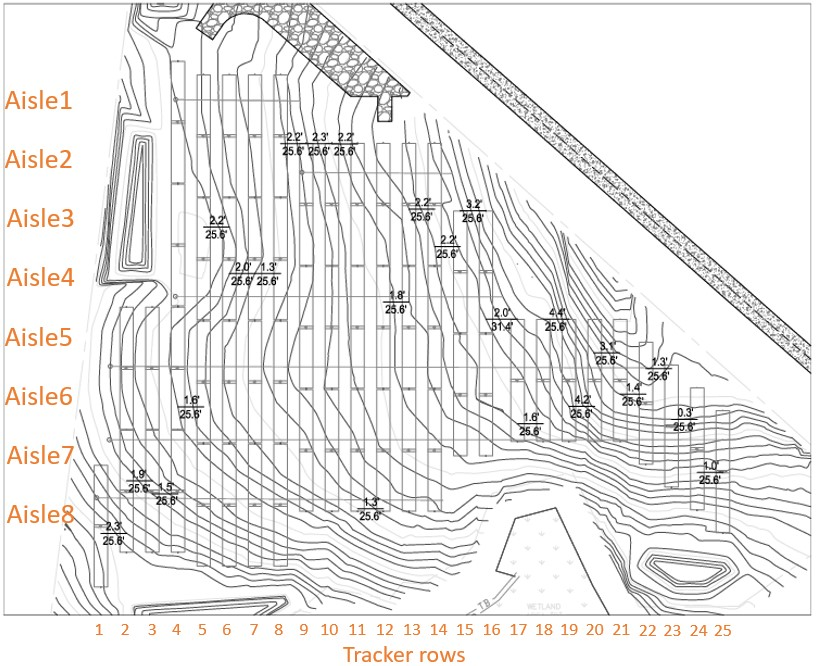
\includegraphics[width=9cm]{Hopewell_Civil_Base.jpg}}
\caption{Contour map of terrain at Hopewell, NC, single-axis array.}
\label{fig:hopewell_contour_map}
\end{figure}

\begin{table}[htbp]
\caption{Summary of East-West Slopes}
\begin{center}
\begin{tabular}{|c|c|c|c|}
\hline
\textbf{Aisle} & \textbf{\textit{Maximum \%}}& \textbf{\textit{Average \%}}& \textbf{\textit{Direction}} \\
\hline
1& 7.81& 6.22& west \\
\hline
2& 7.58& 6.59& west \\
\hline
3& 6.7& 5.77& west \\
\hline
4&5.99& 5.26& west \\
\hline
5& 5.08& 4.28& west \\
\hline
6& 4.69& 3.54& west \\
\hline
7& 4.42& 3.28& west \\
\hline
8& 4.06& 3.99& west \\
\hline
\end{tabular}
\label{table:ew-slope-summary}
\end{center}
\end{table}

\begin{table}[htbp]
\caption{Summary of North-South Slopes}
\begin{center}
\begin{tabular}{|c|c|c|c|}
\hline
\textbf{Row} & \textbf{\textit{Maximum \%}}& \textbf{\textit{Average \%}}& \textbf{\textit{Direction}} \\
\hline
1&  1.76&  1.11& south \\
\hline
5&  2.04&  1.77& south \\
\hline
10& 2.95&  2.54& south \\
\hline
15& 4.81&  4.35& south \\
\hline
20& 6.66&  5.84& south \\
\hline
25& 8.35&  4.96& south \\
\hline
\end{tabular}
\label{table:row-slope-summary}
\end{center}
\end{table}

\subsection{Model Simulation}

The system was modeled using SolarFarmer \cite{Mikofski_8547323} which allows parallel trackers to be oriented on any slope either in a plane ("in-plane" tracker placement) or following the terrain ("follows terrain" tracker placement). Fig.~\ref{tracker-placement} shows these configurations. In-plane represents that the tracker axes in the array form a plane. The plane may have N-S and/or E-W tilt. For illustration purposes, the in-plane example in Fig.~\ref{tracker-placement} only has E-W tilt. In "follows terrain" tracker placement, the tracker axes are not coplanar; the orientation of the tracker axes varies along with the contours of the terrain at a specified height from the ground. In practical design, tracker pile heights can be varied to reduce the undulations of the terrain slopes such that the array slopes formed by the top-of-piles have less variation than the terrain slope.

\begin{figure}[htbp]
\centerline{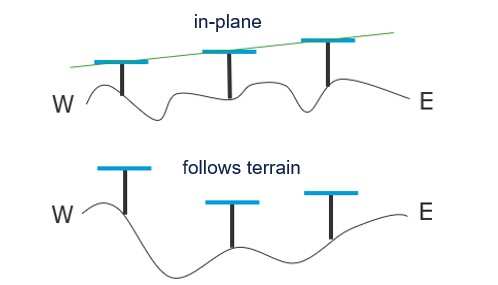
\includegraphics[width=9cm]{tracker-placement.jpg}}
\caption{(Top) "in-plane" tracker placement - the green line guides the eye showing the tracker axes form the same plane. (Bottom) "follows terrain" tracker placement - tracker rows follow terrain contour in N-S and E-W directions.}
\label{tracker-placement}
\end{figure}

Trackers in SolarFarmer can backtrack on any arbitrary slope using standard backtracking or slope-aware backtracking \cite{Anderson2020}. These backtracking algorithms avoid row-to-row shading while minimizing the angle of incidence to maximize output energy. However, this shade avoidance is true only for systems constrained to a plane. In standard backtracking, the array stays shade-free only when installed on flat horizontal ground. In slope-aware backtracking, the array remains shade-free only when the tracker axes are in-plane. In contrast, trackers following the terrain (not in a plane) may shade each other despite backtracking. As shown in Fig.~\ref{terrain-shade} with "follows terrain" tracker placement, row-to-row shading can occur wherever the terrain deviates significantly from the mono-plane that the trackers assume for backtracking calculations. Triangular shadows can occur with N-S and E-W variations from one tracker axis to the next. 

\begin{figure}[htbp]
\centerline{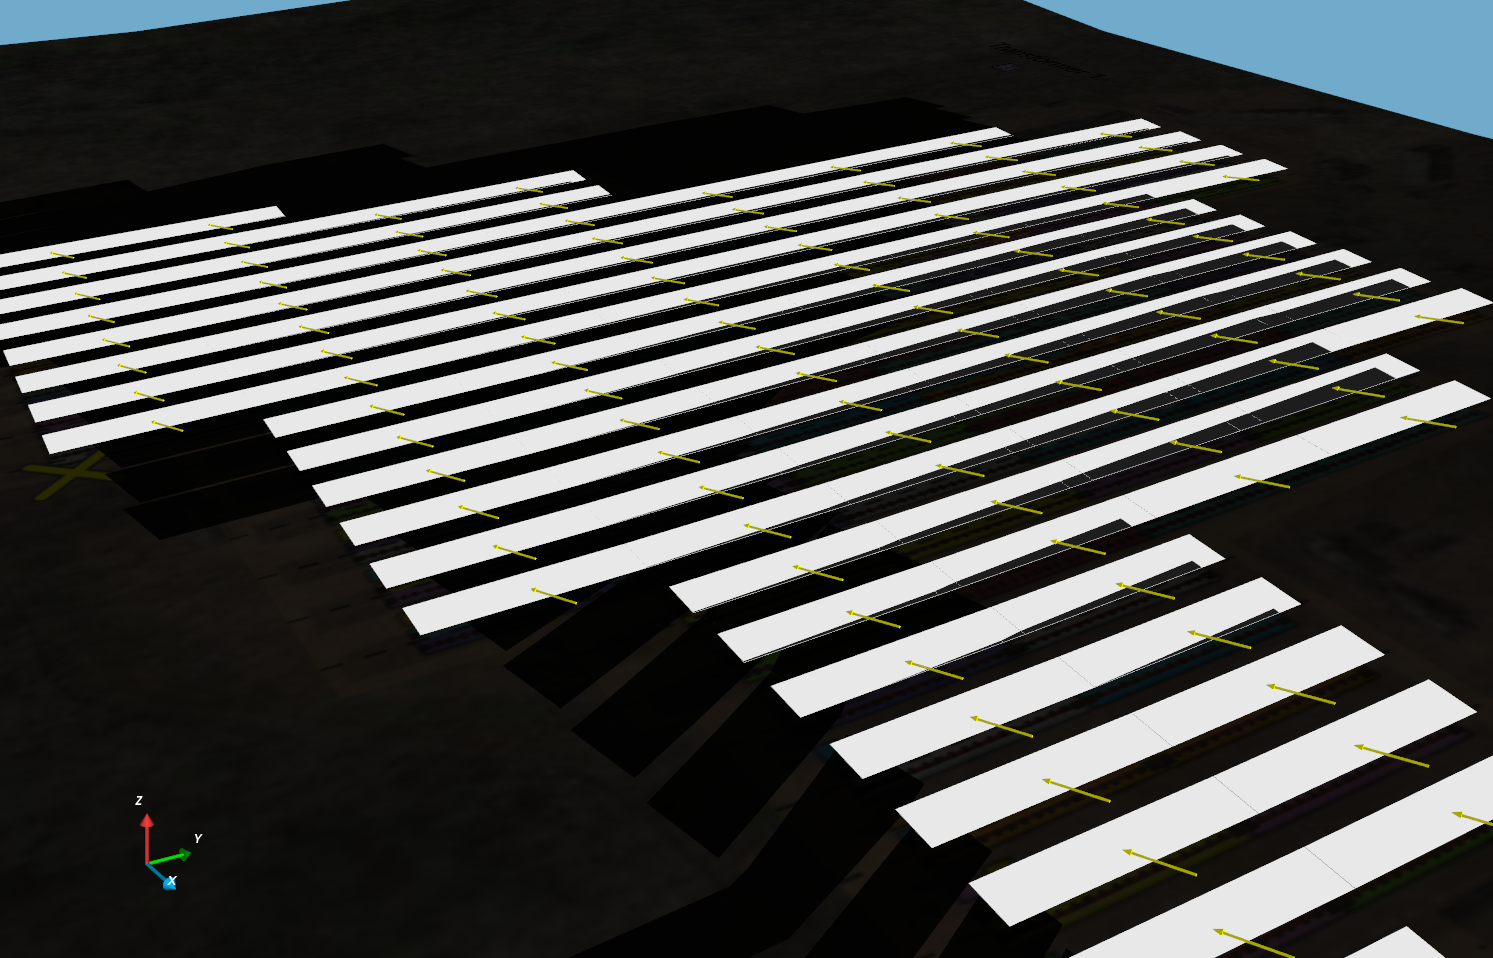
\includegraphics[width=9cm]{Hopewell-Friends-SolarFarmer-shade-follows-std.png}}
\caption{SolarFarmer simulation of row-to-row shading during backtracking for trackers following the sloping terrain at the Hopewell, NC, at 5:40 AM on June 17, 2019. Due to differences in north-south slopes between rows, some shadows are triangular and shade is non-uniform across the array.}
\label{terrain-shade}
\end{figure}

The current version of SolarFarmer offers both 2D and 3D simulations. For this study, 3D simulation was used to allow trackers to follow the terrain. The 3D simulation uses a combination of two techniques to calculate shading on the trackers: a geometric solution to calculate row-to-row shading for the beam component, and a software rasterization approach that renders the scene on “hemicubes” located at the center of each module for the diffuse component. 

The geometric solution uses the sun angles and position of the trackers to determine the shade projection of the the row in front to the row in back in order. The projection determines the shading extent, incident irradiance, and electrical mismatch. From these parameters,  energy output on trackers at any timestep, rotation, and terrain can be calculated. The model does not currently consider shading from arbitrary obstacles or the terrain, but for this study there were no other shading obstacles other than the trackers themselves.

The software rasterization approach (used in the previous paper \cite{Mikofski_9300381}) is required to calculate the diffuse shading component for the trackers. Although less computationally intense than ray-tracing, the software rasterization approach is still more complex than the 2D model, so the complex calculation is simplified by binning the tracker positions at all time-steps into 10° buckets, and each time-step can then be associated with a tracker position bin. The calculation then loops over the typically twelve tracker position bins (+/-60deg tracker rotation angle) and renders the full 3D scene at a representative rotation for the bin. The shading obstacles are then projected onto pixels of each hemicube, and the results are transformed into a cache of shaded or not shaded state for each 1° azimuth and zenith bin for each hemicube. These are then transformed into a diffuse component depending on how much of the sky is visible to each hemicube. A single hemicube at the center of each module was deemed sufficient to determine diffuse sky irradiance incident in the plane of array for the entire module, as the view factor for diffuse sky varies very little on the front side of the module (around 8\% difference between top and bottom according to the 2D model \cite{Mikofski_8980572}). Also, when incorporating the diffuse component in the energy calculation, an average of the individual module diffuse sky irradiances over the site is used per time-step. Along with approximations introduced with the tracker position binning, any finer-resolution hemicube calculations would have little effect on the result.

The combination of these two shading approaches results in a sufficiently accurate solution that runs in an acceptable computation time.

\subsection{Model Site Layouts}

The Hopewell Friends Solar array was first modeled with 111-qty trackers with a total of 222 strings for a total DC size of 1.44-MW, which is slightly smaller than the specified size of 1.45-MW. Second, the site was modeled with 74 inverters, creating a DC/AC ratio less than one, to remove the effects of clipping. The actual site has only 45 inverters and a DC/AC ratio of 1.3. Third, the tracker spacing was made uniform throughout the array with tracker aisles aligned for the model, which differs slightly from the site layout. Finally, the modules were treated as monofacial, because bifacial modeling is currently only possible for 2D simulations and 3D modeling was needed for this study to capture the terrain. These changes were made for ease of modeling and to remove factors such as variable row spacing and other artifacts that could confound the effect of sloped terrain.

Fig.~\ref{fig:layouts} shows the layout sections used for modeling. The array was divided into layouts of varying granularity for simulations. As shown in Table~\ref{table:system-summary}, subdividing the array creates layouts with different orientations, so the systems will track slightly differently. The subdivisions allow parts of the array to be more south-facing with a higher tilt and more southerly azimuth than the 1-layout model. Note that the layout azimuth is the azimuth of the slope, while the tracker axis remains aligned N-S. Each model was then simulated in both tracker placement modes to determine the tracker terrain loss. The "in-plane" mode positions all trackers in the same plane, but may result in some trackers exceeding the maximum specified height above the ground. The "follow terrain" mode positions the trackers at the minimum specified height above ground. The "layout-plane" in Table~\ref{table:system-summary} specifies the orientation plane for the "in-plane" backtracking mode and is also the orientation plane that determines backtracking for "follows terrain" mode. Each model was simulated with both standard \cite{Marion2013} and slope-aware \cite{Anderson2020} backtracking, and both 5-minute and hourly irradiance input, which was obtained from the NREL Physical Solar Model v3 (PSM3) \cite{Sengupta2018}. A total of 24 simulations were performed: 8 runs for each layout (2 placement models, 2 backtracking algorithms, and 2 input data resolutions).

\begin{figure}[htbp]
\centerline{\includegraphics[width=9cm]{layouts.jpg}}
\caption{Sketch of layout sections. The 1-layout model combines Sections 1, 2, and 3; the 2-layout model uses Section 1 as-is and combines Section 2 and 3; the 3-layout model uses each section as-is. Section 1 (54 strings), Section 2 (30 strings), Section 3 (27 strings).}
\label{fig:layouts}
\end{figure}

\begin{table}[htbp]
\caption{Summary Tracker Layouts}
\begin{center}
\begin{tabular}{|c|c|c|c|}
\hline
\textbf{Number of Layouts} & \textbf{\textit{1}}& \textbf{\textit{2}}& \textbf{\textit{3}} \\
\hline
number of trackers&    111& 54&  54 \\
        &     &   57&  30 \\
        &     &     &  27 \\
\hline
layout-plane azimuth (\degree)& 236.9&  247.26&  246.78 \\
       &      &  223.03&  238.47 \\
       &      &        &  207.58 \\
\hline
layout-plane tilt (\degree)&    2.83&    2.92&    2.89 \\
    &        &    2.98&    3.58 \\
    &        &        &    3.26 \\
\hline
tracker axis tilt (\degree)&   1.55&    1.13&    1.14 \\
         &       &    2.18&    1.87 \\
         &       &        &    2.89 \\
\hline
tracker side-slope (\degree)&  2.37& 2.69&    2.66 \\
          &     & 2.03&    3.05 \\
          &     &     &    1.51 \\
\hline
\end{tabular}
\label{table:system-summary}
\end{center}
\end{table}

\subsection{Uneven Terrain DNV Shade Loss Model}
Separate from SolarFarmer, DNV has developed an independent model to estimate tracker terrain loss. The model calculates the energy impact from standard backtracking and slope-aware backtracking on E-W slopes compared to horizontal ground. The model accounts for the shade loss when trackers are facing an E-W upslope and the irradiance loss when the trackers are facing an E-W downslope. The N-S slopes are determined separately, as discussed further below. A post-process model was developed to calculate the row-to-row shade loss for standard tracking and slope-aware tracking, using inputs of E-W ground slope, ground cover ratio (GCR), and PVsyst parameters. Simulations were run in PVsyst across 5 locations with diffuse fractions 0.26-0.5, 3 GCRs (0.3-0.5), and 16 E-W ground slopes (0.1-25\%). The post-processing model was applied to each PVsyst simulation output (hourly data) to calculate the shade losses. From the results of these 240 simulations, two correlation equations were developed which determine shade losses using only 3 factors: diffuse fraction, ground cover ratio, and E-W ground slope. One equation determines the shade loss from standard tracking on E-W slopes and a second equation determines the shade loss from slope-aware backtracking on E-W slope. For the Hopewell Friends site, the equation inputs were diffuse fraction 0.39 and GCR 0.51.

Using US Geographical Survey (USGS) data, the site terrain is analyzed into E-W slope bins. The ground slope is input into the correlation equations to determine the shade losses for each slope bin. Then a weighted average of the slope bins is calculated to derive the overall E-W slope shade losses for standard tracking and slope-aware tracking over the entire site. The weighted average is based on how much area each slope bin constitutes at the site. The USGS data is also analyzed into N-S slope bins to determine the average north-facing slopes and south-facing slopes. The north-facing and south-facing tracker axis tilts can then be applied in PVsyst to determine the N-S slope energy impact.


\section{Results}

The results in this section contain total global incident (GI) insolation in $kWh/m^2$, energy yield in $kWh/kW_p$, the percent of plane of array irradiance lost to shading (diffuse component), and the percent of output lost to electrical mismatch compared to the maximum power point of the array (beam component). These results are used to calculate the tracker terrain loss, using the following formula:

\begin{equation}
\text{Tracker Terrain Loss} = 1 - \frac{Y_\text{terrain}}{Y_\text{horizontal}}\label{eq:tracker-terrain-loss}
\end{equation}

$Y_\text{terrain}$ and $Y_\text{horizontal}$ are the energy yield in $kWh/kW_p$ of the trackers on variable terrain and horizontal ground, respectively. The simulated energy yield for 5-minute input data for standard backtracking on horizontal ground, standard backtracking on terrain, and slope-aware backtracking on terrain is shown in Table~\ref{table:energy-5min}. The corresponding terrain losses compared to horizontal are shown in Table~\ref{table:terrain-loss-5min}.

\begin{table}[htbp]
\caption{Energy Yield for Tracker Layouts for 5-minute Input Data}
\begin{center}
\begin{tabular}{|c|c|c|c|c|c|}
\hline
\textbf{Lay-}& \textbf{\textit{Terrain}}& \textbf{\textit{GI}}&        \textbf{\textit{Yield}}&        \textbf{\textit{Shading}}& \textbf{\textit{Mismatch}} \\
\textbf{outs}& \textbf{\textit{Mode}}&    \textbf{\textit{$kWh/m^2$}}& \textbf{\textit{$kWh / kW_p$}}& \textbf{\textit{\%}}&      \textbf{\textit{\%}} \\
\hline
\multicolumn{6}{|c|}{\textit{Standard backtracking}} \\
\hline
1& Horiz.& 2024.1&  1662.1& 3.1& 0 \\
\hline
2& Horiz.& 2024.1&  1663.5& 3.0& 0 \\
 \hline
3& Horiz.& 2024.1&  1664.8& 2.9& 0 \\
\hline
\multicolumn{6}{|c|}{\textit{Standard backtracking}} \\
\hline
1& In Plane& 2044.0&  1628.6& 2.6& 3.4 \\
 & Follow&         &  1625.8& 2.7& 3.4 \\
\hline
2& In Plane& 2045.4&  1632.9& 2.6& 3.2 \\
 & Follow&         &  1631.8& 2.6& 3.2 \\
\hline
3& In Plane& 2046.5&  1637.1& 2.6& 3.1 \\
 & Follow&         &  1636.4& 2.6& 3.1 \\
\hline
\multicolumn{6}{|c|}{\textit{Slope-aware backtracking}} \\
\hline
1& In Plane& 2044.9&  1700.0& 1.9& 0 \\
 & Follow&         &  1658.9& 2.1& 2.1 \\
\hline
2& In Plane& 2046.3&  1700.3& 1.9& 0 \\
 & Follow&         &  1668.3& 2.0& 1.7 \\
\hline
3& In Plane& 2047.3&  1701.8& 1.9& 0 \\
 & Follow&         &  1673.9& 2.0& 1.5 \\
\hline
\end{tabular}
\label{table:energy-5min}
\end{center}
\end{table}


\begin{table}[htbp]
\caption{Tracker Terrain Loss for 5-minute Input Data}
\begin{center}
\begin{tabular}{|c|c|c|}
\hline
\textbf{Lay-}& \textbf{\textit{Standard}}& \textbf{\textit{Slope-aware}} \\
\textbf{outs}& \textbf{\textit{backtrack}}&    \textbf{\textit{backtrack}}\\
\hline
\multicolumn{3}{|c|}{\textit{In-plane}} \\
\hline
1& -2.0\% & +2.3\% \\
\hline
2& -1.8\% & +2.2\% \\
\hline
3& -1.7\% & +2.2\% \\
\hline
\multicolumn{3}{|c|}{\textit{Follows terrain}} \\
\hline
1& -2.2\% & -0.2\%  \\
\hline
2& -1.9\% & +0.3\%  \\
\hline
3& -1.7\% & +0.5\%  \\
\hline
\end{tabular}
\label{table:terrain-loss-5min}
\end{center}
\end{table}

Due to the west-facing slope, standard backtracking will lead to shading and electrical losses in the morning because the array needs to backtrack more at a flatter angle to avoid shade. In the afternoon, irradiance losses will be present because the tracker starts moving away from the sun prematurely when the array can be at a steeper angle without shade. In Table~\ref{table:terrain-loss-5min}, the second column shows that standard backtracking incurs -1.7-2.2\% tracker terrain loss. The in-plane and follows terrain results were similar; this observation might indicate that for standard backtracking, the E-W slope shade loss was dominant over shade irregularities that are produced by follows terrain compared to in-plane tracker placement (i.e. triangular shadows).

In contrast to standard backtracking, slope-aware backtracking accounts for planar ground slopes, leading to improved performance over standard backtracking. Slope-aware backtracking eliminates E-W shading for trackers on uniform, non-horizontal planes. This behavior can be seen from Table~\ref{table:energy-5min} with 0\% electrical mismatch loss for in-plane slope-aware backtracking. The difference between in-plane and follows terrain (1.5-2.1\%) illustrates that slope-aware backtracking can avoid shade when the tracker axes are coplanar, but shade will still occur when non-planar tracker axes are on variable terrain. The result suggests that putting the tracker axes in the same plane as much as possible (removing undulations in terrain) and using slope-aware backtracking will maximize energy yield.

Considering slope-aware tracker terrain losses, the last column in Table~\ref{table:terrain-loss-5min} has positive values indicating tracker terrain \textit{gains} compared to horizontal. As the site is in the northern hemisphere, the sun is to the south, and the south-facing slope of the site will produce an energy gain compared to horizontal. Follows terrain slope-aware backtracking has a +2\% improvement compared to standard backtracking, essentially recovering the standard backtracking E-W shade losses. In addition, in-plane slope-aware backtracking has a +2\% improvement over follows terrain slope-aware backtracking. The in-plane slope-aware backtracking has an additional advantage over follows terrain because in-plane placement has an entirely south-facing tilt. On the other hand, follows terrain slope-aware backtracking is subject to some parts of the array with north-facing tilt and shade irregularities. 

The same simulations for 5-minute input data were performed for 1-hour input data. To explore the N-S impact compared to horizontal further, an additional simulation was performed for a layout plane with N-S tilt but no E-W slope ("no E-W"). The energy yield from the 1-hour data simulations are shown in Table~\ref{table:energy-1hr}. The south-facing tilt with no E-W plane ("no E-W") had a +2\% gain compared to horizontal ground. This result aligns with the +2.1-2.2\% gain of in-plane slope-aware backtracking compared to horizontal. The slope-aware backtracking in-plane benefits from a +2\% boost from an entirely south-facing array compared to horizontal, while also recovering +2\% E-W shade loss from standard backtracking. 

The corresponding 1-hr data of tracker terrain losses compared to horizontal ground is shown in Table~\ref{table:terrain-loss-1hr}. Evaluating this 1-hour data with the 5-minute data in Table~\ref{table:terrain-loss-5min}, the results were similar. The 1-hour data had a small increase in output and global incident irradiance. A separate study which is to be presented later this year will examine this issue more closely.

\begin{table}[htbp]
\caption{Energy Yield for Tracker Layouts for 1-Hour Input Data}
\begin{center}
\begin{tabular}{|c|c|c|c|c|c|}
\hline
\textbf{Lay-}& \textbf{\textit{Terrain}}& \textbf{\textit{GI}}&        \textbf{\textit{Yield}}&        \textbf{\textit{Shading}}& \textbf{\textit{Mismatch}} \\
\textbf{outs}& \textbf{\textit{Mode}}&    \textbf{\textit{$kWh/m^2$}}& \textbf{\textit{$kWh / kW_p$}}& \textbf{\textit{\%}}&      \textbf{\textit{\%}} \\
\hline
\multicolumn{6}{|c|}{\textit{Standard backtracking}} \\
\hline
1& Horiz.& 2029.6&  1668.7& 3.1& 0 \\
 & No EW & 2049.9&  1707.2& 1.8& 0 \\
\hline
2& Horiz.& 2029.6&  1670.0& 3.0& 0 \\
 & No EW & 2051.5&  1703.9& 2.1& 0 \\
\hline
3& Horiz.& 2029.6&  1671.4& 2.9& 0 \\
 & No EW & 2052.7&  1706.3& 2.0& 0 \\
\hline
\multicolumn{6}{|c|}{\textit{Standard backtracking}} \\
\hline
1& In Plane& 2049.9&  1628.9& 2.8& 3.6 \\
 & Follow&         &  1631.1& 2.6& 3.6 \\
\hline
2& In Plane& 2051.5&  1635.0& 2.7& 3.4 \\
 & Follow&         &  1635.9& 2.6& 3.4 \\
\hline
3& In Plane& 2052.7&  1639.8& 2.6& 3.2 \\
 & Follow&         &  1640.3& 2.6& 3.2 \\
\hline
\multicolumn{6}{|c|}{\textit{Slope-aware backtracking}} \\
\hline
1& In Plane& 2048.7&  1704.7& 1.9& 0 \\
 & Follow&         &  1662.1& 2.1& 2.2 \\
\hline
2& In Plane& 2050.2&  1705.0& 2.0& 0 \\
 & Follow&         &  1672.3& 2.1& 1.8 \\
\hline
3& In Plane& 2051.1&  1706.4& 1.9& 0 \\
 & Follow&         &  1678.1& 2.0& 1.5 \\
\hline
\end{tabular}
\label{table:energy-1hr}
\end{center}
\end{table}


\begin{table}[htbp]
\caption{Tracker Terrain Loss for 1-Hour Input Data}
\begin{center}
\begin{tabular}{|c|c|c|}
\hline
\textbf{Lay-}& \textbf{\textit{Standard}}& \textbf{\textit{Slope-aware}}\\
\textbf{outs}& \textbf{\textit{Backtrack}}&    \textbf{\textit{Backtrack}} \\
\hline
\multicolumn{3}{|c|}{\textit{In-plane}} \\
\hline
1& -2.4\% & +2.2\%  \\
\hline
2& -2.1\% & +2.1\%  \\
\hline
3& -1.9\% & +2.1\%  \\
\hline
\multicolumn{3}{|c|}{\textit{Follows terrain}} \\
\hline
1& -2.3\% & -0.4\%  \\
\hline
2& -2.0\% & +0.1\%  \\
\hline
3& -1.9\% & +0.4\%  \\
\hline
\end{tabular}
\label{table:terrain-loss-1hr}
\end{center}
\end{table}

The last component of this study was to examine whether subdividing the array would decrease tracker terrain loss. The arrays were split into multiple layouts each with their own N-S axis tilt and E-W slope. In general for this site, splitting the site into 3 layouts reduced tracker terrain loss by roughly 0.5\%. However, more important is that in-plane trackers are needed for maximum performance. Splitting the array into layouts each with their own axis tilt and cross-axis slope can minimize the amount of cut and fill required to build the site by decreasing the range of pile heights to constrain the tracker axes all to the same plane.

\subsection{Uneven Terrain DNV Shade Loss Model}
Based on the site slope analysis, the site area is 68\% facing south (2.8\degree  slope) and 32\% facing north (1.2\degree  slope). The E-W effective slope was calculated to be 4.3\%, which is consistent with the site characterization in Table~\ref{table:ew-slope-summary}. 

The results of the DNV terrain shade loss model are shown in Table~\ref{table:uneven-terrain}. Considering both E-W and N-S slopes, the tracker terrain loss was estimated to be \textminus2.1\% for standard backtracking and +0.7\% for slope-aware backtracking compared to horizontal ground. The N-S slope impact contributed a +1.1\% gain, considering a weighted average of the north-facing 32\% and south-facing 68\% parts of the array. A separate calculation was also performed for an entirely south-facing layout (no E-W component) and resulted in a +2\% gain compared to horizontal. This result is similar to the SolarFarmer "no E-W" result compared with horizontal.    

The DNV shade loss model results aligned well with the tracker terrain loss calculated by SolarFarmer. The DNV model standard backtracking had -3.2\% E-W shade impact, similar to the mismatch loss from standard backtracking in SolarFarmer of -3.2-3.6\% across in-plane and follows terrain cases. For slope-aware backtracking, the DNV model showed almost complete recovery of the E-W slope impact (-0.4\%), similar to the 0\% in-plane slope-aware mismatch loss in SolarFarmer. When including both E-W and N-S slope impacts compared to horizontal, slope-aware backtracking has a +2-3\% benefit over standard backtracking in both the DNV model and SolarFarmer follows terrain model. The SolarFarmer in-plane slope-aware model has an additional +2\% boost for the entirely south-facing tilt compared to horizontal.    

Overall, standard backtracking terrain impact was \textminus2.1\% in the DNV model, while SolarFarmer follows terrain resulted in \textminus1.7-2.3\%. Slope-aware backtracking for the DNV model resulted in more energy gain, +0.7\% compared to SolarFarmer's \textminus0.4\% to +0.5\%. Note that DNV considers the +0.7\% to be an ideal shade recovery case. In practical application in the field, DNV estimates custom, non-standard backtracking to recover only 70\% of the ideal case based on limited field data. When this practical factor is applied, the DNV model for slope-aware backtracking leads to a tracker terrain loss of +0.5\%, which closely aligns with the SolarFarmer result.

\begin{table}[htbp]
\caption{Tracker Terrain Loss DNV Model}
\begin{center}
\begin{tabular}{|c|c|c|c|}
\hline
\textbf{Energy impact}& \textbf{\textit{Standard}}& \textbf{\textit{Slope-aware}} \\
  & \textbf{\textit{Backtrack}} & \textbf{\textit{Backtrack}} \\
\hline
E-W slope impact & -3.2\% & -0.4\% \\
\hline
N-S slope impact  & \multicolumn{2}{|c|}{+1.1\%}\\
\hline
Net terrain impact & -2.1\% & +0.7\% \\
\hline
\end{tabular}
\label{table:uneven-terrain}
\end{center}
\end{table}

\section{Conclusions}
The Hopewell Friends Solar power plant was simulated with SolarFarmer to calculate tracker terrain loss. This site has variable terrain and an average 4\% southwest slope. The study examined tracker terrain loss using different time intervals, tracker placement, array subdivisions, and backtracking algorithms. With standard backtracking, the tracker terrain loss from SolarFarmer was -1.7-2.4\% when compared to horizontal across array subdivisions and tracker placement models. Dividing the site into more layouts led to tracker terrain losses approximately 0.5\% lower than a single layout. The simulations were repeated with 5-minute and 1-hour input data, but the tracker terrain loss change was marginal. The simulations were also repeated with slope-aware backtracking, which indicated that the tracker terrain loss for this particular site was predominantly caused by the E-W slope and therefore recoverable with slope-aware backtracking. The site has a south-facing tilt which contributes an energy gain. The slope-aware follows terrain had tracker terrain losses of -0.4\% to +0.4\%. The SolarFarmer results were also compared with an independent DNV terrain shade loss model. The DNV model yielded -2.1\% net terrain impact from standard backtracking and +0.7\% compared to horizontal, results which are similar to SolarFarmer. This site had a mostly southwest slope and further work is needed to study tracker terrain losses at more sites, especially those with more complex terrain. In addition, field data of custom backtracking is currently limited in the industry and should be examined to determine how it compares with simulations.

\section*{Acknowledgment}

Data and layout specifications for the Hopewell Friends Solar array were provided by PV Evolution Labs and Cypress Creek Renewables based on funding by the U.S. Department of Energy office of Energy Efficiency and Renewable Energy as detailed in the funding opportunity announcement, DE-FOA-0001840 \cite{CypressCreekRenewables2019}.

\bibliographystyle{IEEEtran}
% argument is your BibTeX string definitions and bibliography database(s)
\bibliography{IEEEabrv,bibliography}

\end{document}
